Numerous different groups have developed overlapping software for fast algorithms. For FMMs, leading analytical impelementations include the single-node multithreaded, `FMM3D' and `FMM2D' \cite{fmm3d, fmm2d}, and the MPI accelerated  `ExaFMM' \cite{exafmm} packages. The ExaFMM project have also developed a single-node multithreaded kernel-independent FMM, `ExaFMM-T' \cite{wang2021exafmm}. For algebraic methods, the landscape is sparser, with few parallel implementations. The standouts being the MPI accelerated `STRUMPACK' \cite{ghyselsstrumpack}, for HODLR and HSS matrices, the multithreaded single-node `FLAM' \cite{ho2020flam}, which supports algorithms for $\mathcal{H}^2$ matrices and the single-node multithreaded $\mathcal{H}^2$-lib software \cite{h2lib2016github}. The majority of codes, except FLAM which is written in Matlab, are written in compiled languages, either Fortran, C or C++, with a minority supporting interfaces to higher level languages \cite{wang2021exafmm,fmm3d}.

We compare these softwares for the calculation of (\ref{eq:ch_2:two_box_calc}) with $N$ randomly distributed particles placed in a unit cube, $[0, 1]^3$, with uniform charge, $q_i=1$, in figure (\ref{fig:ch_3:software_comparison}) \footnote{Our experiments are available at \url{https://github.com/skailasa/phd-thesis/code/}}. Experiments are taken on a single-node AMD Ryzen Threadripper 3970X 32 core processor with 250GB of memory. To avoid thread oversubscription in STRUMPACK and ExaFMM, both designed for multi-node systems, the maximum number of OpenMP threads is restricted to one. Each FMM software is run with an expansion order $P=10$, and the algebraic software's parameters are adjusted to match this level of accuracy. In our algebraic software experiments we exclude $\mathcal{H}^2$-lib from the comparison in figure (\ref{fig:ch_3:software_comparison}) due to constraints on time, restricting our study FLAM, which we used to develop our fast direct solver code in chapter \ref{chpt:7:fds}, and STRUMPACK which is the leading MPI-parallelised code.

In comparing these softwares we aimed to emulate the workflow of a typical user evaluating the differences between software packages, and therefore restricted our study to runs which converged in less than 30 minutes, $\approx 2 \times 10^3$ s. Figure (\ref{fig:ch_3:software_comparison}a) plots the time to compute (\ref{eq:ch_2:two_box_calc}), including the time to create all required data structures. For FLAM this includes the time to factorise and store its explicit hierarchical matrix representation of (\ref{eq:ch_2:two_box_calc}) which is a requirement of the software. Strictly speaking, STRUMPACK's HSS and HODLR matrices are not applicable to (\ref{eq:ch_2:two_box_calc}), as it is a strongly admissable problem. Furthermore the default running mode of STRUMPACK uses randomised sampling, which repeatedly multiplies a given dense input matrix with a randomly generated matrix in order to estimate its compressed form. This leads to a $O(N^2r)$ complexity, where $r$ is a maximum rank of a low-rank block based on a user defined tolerance, when calculating the HSS or HODLR representations. We see the effects of this in super-quadratic factorisation times for increasing $N$. The slow compression can be tuned by a user defined `fast' matrix vector product for low-rank sub blocks of the matrix which could use a low-rank decomposition such as a multipole type expansion, or a purely numerical scheme such as an SVD, to compress these sub-blocks, however we evaluate the software as presented. We observe that FLAM and STRUMPACK, run in its default setting, are impractical for computing even moderately sized matrix vector products, i.e. $N \geq O(10^5)$. With runtimes times for factorisation exceeding our imposed limit of $2 \times 10^3$ s. Unless a hierarchical matrix representation is expressly required, such as for the development of a fast direct solver, we think it is unlikely that a typical user would attempt to optimise STRUMPACK's matrix vector product, as the FMM software tested beat both algebraic softwares by several orders of magnitude in runtime out of the box. Thus making it considerably faster in terms of development time to use these to develop an iterative solver, or evaluate fast matrix vector products.

\begin{figure}
    \begin{tabular}{cc}
        \subfloat[\centering Total Runtime]{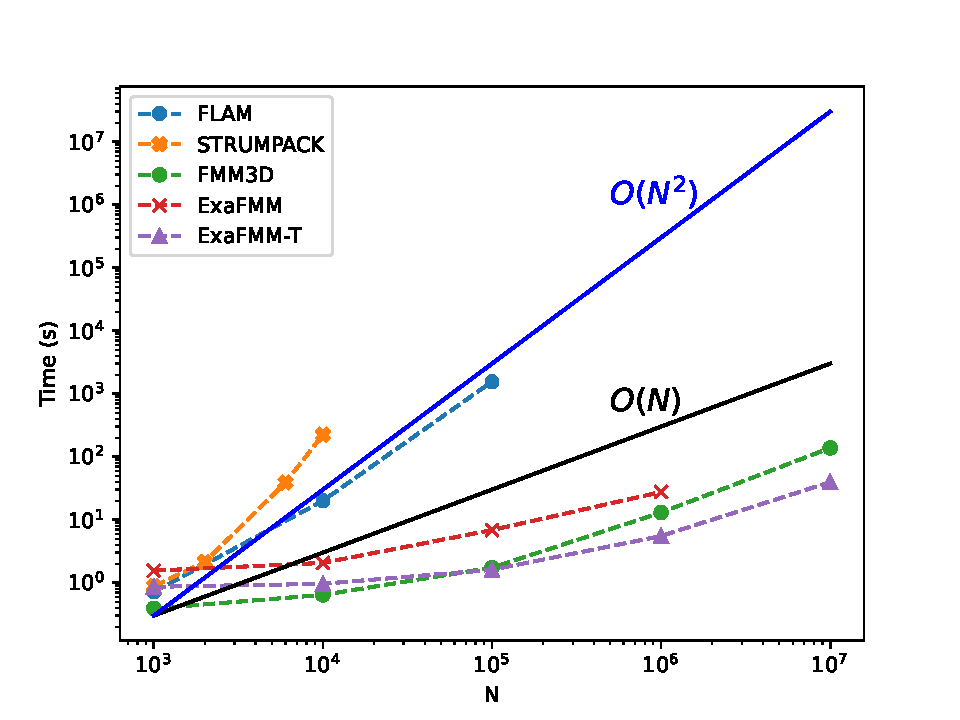
\includegraphics[width=75mm]{ch_3/runtime.pdf}} & \subfloat[\centering Peak Memory Usage]{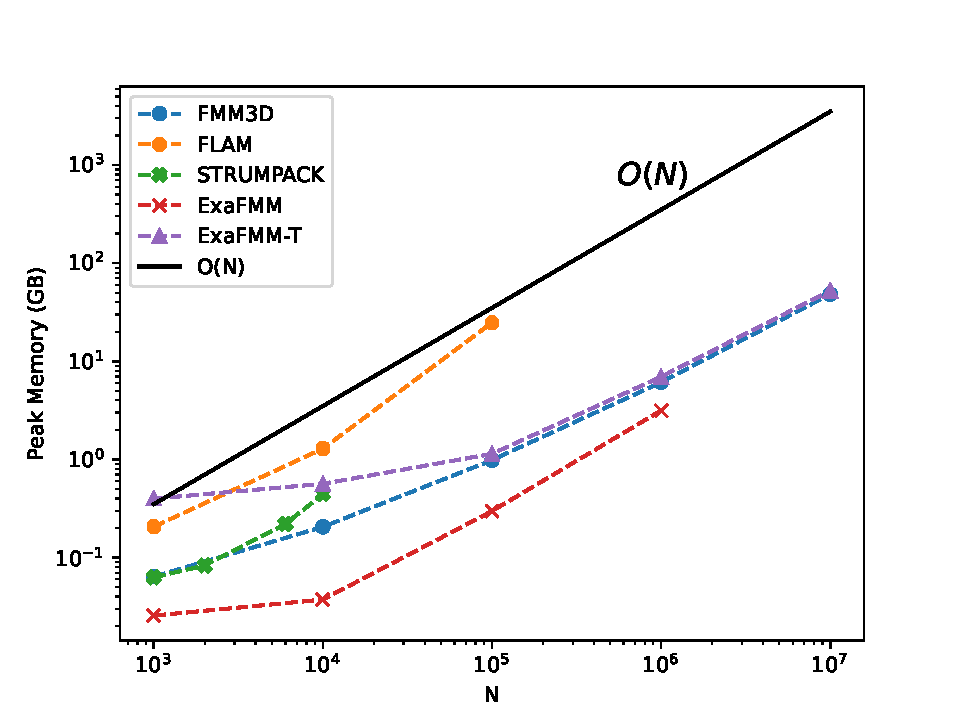
\includegraphics[width=75mm]{ch_3/memory.pdf}}
    \end{tabular}
    \centering \subfloat[\centering Matrix vector product time for algebraic methods.]{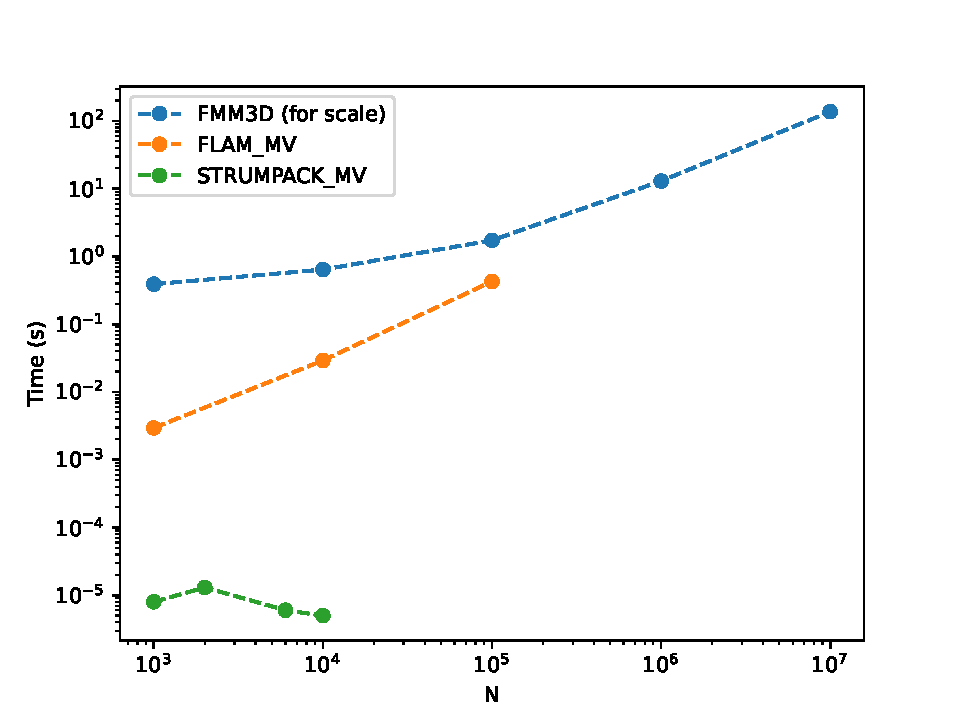
\includegraphics[width=75mm]{ch_3/alg_matvec.pdf}}
    \caption{Comparison of parallel software for fast algorithms, used to calculate (\ref{eq:ch_2:two_box_calc}). Simulations were compared for convergence times $\leq 2 \times 10^3$ s that could fit into memory.}
    \label{fig:ch_3:software_comparison}
\end{figure}

As expected from theory, the analytical FMMs, ExaFMM and FMM3D, consume less memory than the black box ExaFMM-T (fig. (\ref{fig:ch_3:software_comparison}b)). However, for larger problem sizes this difference is marginal between FMM3D and ExaFMM-T. For the largest problem size tested, $N=10^7$, ExaFMM-T is roughly 3.5 times faster than FMM3D with a similar memory footprint. Counter intuitively, the analytical ExaFMM fails to converge in our experiments for $N=10^7$, as its memory requirements exceed the available 250 GB. 

Theoretical considerations aside, each software's performance is practically determined by the computational and algorithmic performance optimisations they take. ExaFMM-T for example uses optimized algorithms for the calculation of inverse square roots \cite{malhotra2015pvfmm}, as well as using SIMD vectorisation for kernel evaluations \cite{wang2021exafmm}. Similarly by stacking $T^{M2L}$ as in (\ref{eq:ch_2:m2l_stacked}), they optimise cache-reuse. Similar SIMD vectorisations are implemented by FMM3D and ExaFMM, however their remaining optimisations are presented opaquely, making it difficult for users to evaluate their relative merits. It is unclear from STRUMPACK's documentation as to whether they use SIMD vectorisations to accelerate kernel evaluations, however they do offer limited GPU offloading but not for algorithms defined on HSS or HODLR matrices. FLAM is multithreaded, however is written for implementation simplicity and algorithm testing and is largely unoptimised for HPC.

Usability, defined in terms of quality of API documentation, available descriptions of mathematical and software optimisations,  quality of software engineering in terms of self-documenting and well commented code, as well as ease of installation, is as critical to the dissemination of scientific software as raw performance. It's unlikely that a user will incorporate a performant piece of software into their work if it's not usable. In this respect FMM3D and ExaFMM-T standout, with well documented APIs, code examples, as well as wrappers to call functionality from higher level languages. STRUMPACK, though relatively well documented, does not support wrappers to higher-level languages. Written in C++, its documentation is largely a description of its object hierarchy, with few examples documenting real world use cases. ExaFMM on the other hand is poorly documented, with few tests or comments, and no wrappers to high-level languages. FLAM, written in Matlab, is easy to install with numerous code examples as well as good documentation. Most softwares, except STRUMPACK which is distributed via the SPACK package manager and FLAM which is a Matlab package, have traditional source builds based on CMake and Make. Local installation can therefore be challenging when building on non-traditional HPC operating systems such as Windows and MacOS.

From the experiments in figure (\ref{fig:ch_3:software_comparison}) it's clear that software choice can have dramatic impact on runtime and memory scaling regardless of algorithmic choice. However software choice is unlikely to be purely guided by performance considerations, as we have seen each example software have different levels of user support in terms of example code, documentation and code comments, and thus have different practical usability. For the Laplace problem of (\ref{eq:ch_2:two_box_calc}) all softwares can be used more or less out of the box, however oscillatory Helmholtz kernels are only natively supported by a few \cite{exafmm,wang2021exafmm,fmm2d, fmm3d}. The most complete functionality, with the addition of Stokes and Maxwell kernels, are only supported by FMM2D and FMM3D. From a non-expert user's perspective, merely understanding the theory behind each algorithm isn't enough to expect a guaranteed performance, as demonstrated by the different memory requirements of the analytical FMMs. In light of this, users would likely be tempted to pick a `median' option, which guarantees good performance, scalability, easy installation, and usability via a high-level language wrapper and support for multiple problems. This makes FMM2D and FMM3D the standout options, however as they're developed as a high-performance Fortran libraries, they are relatively unmalleable, with a steep learning curve for potential contributors and are unfortunately limited to single-node systems.

\subsection*{Conclusion}

We identify a distinct lack of software for fast algorithms that fulfills our usability criteria and can also scale to multi-node systems. Presently available software is not composable, with differing APIs and re-implementations of high-performance kernels as well as data structures such as quad and octrees. Wrappers for high-level languages are not uniformly available, and builds can be challenging in non-Linux environments. We aim to solve this with our proposed software infrastructure, the high-level architecture of which is illustrated in figure (\ref{fig:ch_3:rusty_roadmap}). By offering a set of composable libraries with a unified API for FMMs and algebraic methods for constructing matrix inverses, we aim to maximally re-use highly-optimised code, such as for SIMD vectorised kernel evaluations, and quad and octrees that can scale across multiple processors. 

We initially explored Python, in conjunction with high-performance `just in time' (JIT) code generation tool Numba \cite{lam2015numba}, as a base programming model for our infrastructure. We document this through our experience building a Python based KIFMM in chapter \ref{chpt:4:pyexafmm}. Although we evaluate a single code-generation tool, Numba, we believe our experience generalises to other approaches that rely on similar JIT compiled technologies for the acceleration of code written in high-level languages, such as Julia. We found the constraints placed on our software using this approach to be too restrictive for the infrastructure we were planning and therefore pivoted to Rust, a modern compiled language designed explicitly with code portability in mind, as the base language of our infrastructure.  We believe that Rust offers a powerful and productive alternative to older compiled languages for the development of scientific software, with similar runtime performance. We explore its beneficial properties in chapter \ref{chpt:5:rust}. Most important of these is its build system, Cargo, which is specified by a simple TOML file. This makes it easy to deploy Rust codes on most common platforms without the need for complex build CMake style build scripts. With users able to develop software locally, before deploying to a cluster, while being able to expect high-performance performance. Rust's syntax inherits from both functional and imperative paradigms, and its trait system wholly replaces object orientation, making the description of shared behaviour, and data oriented programming, significantly more readable. Importantly, it is also easy to develop wrappers from Rust to Python using its C foreign function interface \cite{maturin2022github}, making it easy for novice programmers to develop and deploy our solvers on a range of devices, from their laptops to supercomputing clusters. This combined Rust and Python approach combines the usability and portability features we are looking for, commonly associated with interpreted languages, with the performance of more complex compiled languages such as C++.

\begin{figure}
    \centerline{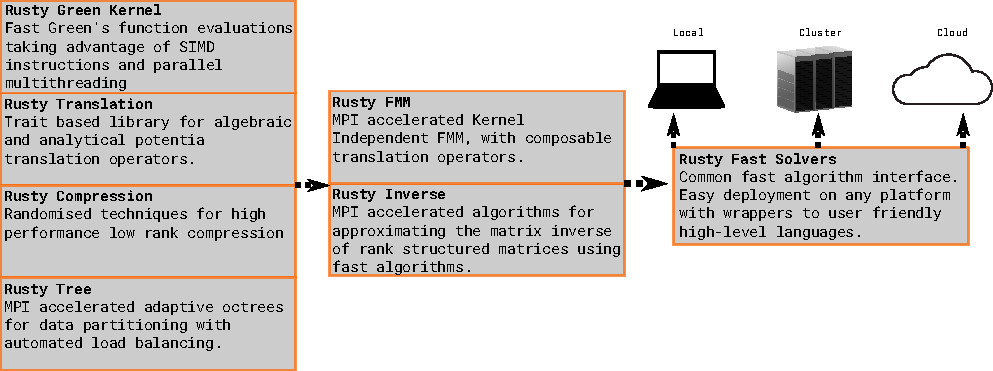
\includegraphics {ch_3/rusty_roadmap.pdf}}
    \caption{Hierarchy of our proposed infrastructure, with key functionality separated into individual libraries we maximise code re-use across projects. Once completed using Rust's code generation infrastructure, users will be able to deploy our software from desktop workstations, to supercomputing clusters and expect scalable high-performance code, while being able to write application code in Python.}
    \label{fig:ch_3:rusty_roadmap}
\end{figure}
